\documentclass[12pt]{article}
\usepackage{amssymb,amsmath,graphicx,mathtools}
\usepackage{listings}
\usepackage[margin=0.75in]{geometry}
\parindent 16 pt
\usepackage{fancyhdr}
\usepackage[hidelinks]{hyperref}
\usepackage[usenames,dvipsnames]{xcolor} % Required for custom colors
\usepackage{listings}
\usepackage{float}
\usepackage{sectsty}
%\pagestyle{fancy}
%\fancyhead[R]{Imad Ali}
%\fancyhead[L]{Bayesian Win Probability in Basketball}
\DeclarePairedDelimiter\ceil{\lceil}{\rceil}
\DeclarePairedDelimiter\floor{\lfloor}{\rfloor}

\sectionfont{\sffamily\bfseries\upshape\large}
\subsectionfont{\sffamily\bfseries\upshape\normalsize}
\subsubsectionfont{\sffamily\mdseries\upshape\normalsize}

\definecolor{links}{HTML}{FF6688}

\lstset{
    language=R,
    basicstyle=\scriptsize\ttfamily,
    stepnumber=1,
    numbersep=5pt,
    showspaces=false,
    showstringspaces=false,
    showtabs=false,
    frame=single,
    tabsize=2,
    captionpos=b,
    breaklines=true,
    breakatwhitespace=false,
    escapeinside={},
    keywordstyle={},
    morekeywords={}
    }

\title{Nothing as it seems - A Bayesian inference alternative to statistical significance}
\author{Imad Ali\thanks{National Basketball Association} \and Jonah Gabry\thanks{Columbia University}}

\begin{document}
\maketitle
\abstract{\noindent This paper outlines common misconceptions of Frequentist statistical significance and proposes a more intuitive Bayesian alternative. At a high-level Frequentist methods focus on the distribution of the test statsitic as opposed to the parameter of interest, whereas the methods proposed here allow the researcher to perform inference directly on the parameter of interest.}
\tableofcontents
\newpage
% CaUSTOM SHORTCUTS

\def\ci{\perp\!\!\!\perp}
\def\ex{\mathbb{E}}
\def\prob{\mathbb{P}}
\def\ind{\mathbb{I}}
\def\grad{\triangledown}
\def\bigo{\mathcal{O}}

\section{Introduction}

Some literature reviewy stuff. \\

\noindent In the following section we discuss common misconceptions surrounding test statistics, p-values, and generally speaking the misuse of the term statistical significance. We then show an alternative approach under the Bayesian framework to evaluate significant differences in parameters. Finally, we extend this to how we can deal with the significance of parameters in generalized linear regression models. \\

\subsection{Misinterpreting statistical significance}

\noindent A quantity is defined to be statistically significant if the test statistic computed with this quantity is unlikely to occur under the null hypothesis, where the null hypothesis assumes that there is no material difference between two quantities. What this means is that if we repeatedly draw samples of data from the population under the null hypothesis, compute the same statistic, and plot the empirical distribution of the statistic; then the statistic we computed from our original data would fall somewhere in the tails (i.e. a low probability region). One way to quantify this is to compute the proportion of the distribution that is in the tails from the computed test statistic. This quantity is known as a p-value and tells you the probability of computing a statistic under the null hypothesis that is as extreme as the one at hand. Lower p-values indicate that the computed test statistic is way out in the tail(s) of the distribution. \\

\noindent In this discussion of statistical significance we have been talking about quantities that we, as applied researchers, are not really interested in; test statistics and p-values. We are more interested in the underlying quantities used to compute these statistics. It would be more appropriate to do inteference on quantities that we are actually interested in compared to statistics derived from these quantities. \\

\section{Difference in parameters}

This section outlines how Bayesian inference can be performed as an alternative to statistical significance. It is easier to talk about the process of inference in context so we use alternatives to the t-test and binomial test as examples below. In all examples we will perform the canonical frequentist method of determining statistical significance and then show a Bayeisan alternative by modeling the data using \textbf{rstan}, the R interface to the Stan probabilistic programming language. \\

\subsection{t-Test: Difference between empirical mean an hypothesized value}

A one sample t-test is used to test the whether the mean of a sample of data $\bar{x}$ is significantly different from some hypothesized value $\mu$. The test statistic assumes that data $x$ is generated from the normal distribution and is calculated as,

$$
\mbox{t-statistic} = \frac{\bar{x}-\mu}{\sigma/\sqrt{n}}
$$

\noindent where $\sigma$ is the standard deviation of the data $x$ and $n$ is the sample size of the data. This statistic follows the t-distribution with $n-1$ degrees of freedom.

\noindent Below we have a sample of ten observations generated from $\mathcal{N}(4.5,2)$.

\begin{verbatim}
  x <- c(5.820883, 2.667825, 3.332511, 3.388233, 7.976444,
         5.925112, 6.465919, 7.064625, 3.012066, 2.771472)
\end{verbatim}

\noindent Suppose we want to test whether the mean of these observation is statistically different from $\mu = 4.5$. This is what is known as a two-tailed test since we are interested in determining whether the mean is significantly greater than 4.5 or significantly less than 4.5. Applying the formula to the data gives the following t-statistic,

$$
\frac{4.84-4.5}{2.01/\sqrt{10}} \approx 0.5394
$$

\noindent Since we are dealing with a two-tailed test our test statistics of interest are $\mid 0.5394 \mid$ and $-\mid 0.5394 \mid$. As mentioned in the introduction, we want to determine how unlikely it is to compute test statistics more extereme than the ones we have computed. We can do this using the cumulative distribution function for the t-distribution $\Phi(\mu, \nu)$ parameterized by location $\mu$ and degrees of freedom $\nu$. Since the t-distribution is symmetric we can compute the probability of calculating a statistic less than or equal to -0.5394 under the null hypotheis and multiply this value by 2. Performing this computation yields,

$$
2 \cdot \Phi(0.5394, 10-1) \approx 0.6027
$$

\noindent So there is about a 0.6 probability that a test statistic could occur that is more extereme than the one we computed. In other words, if we repeatedly randomly sample 10 observations under the null hypotheis $x \sim \mathcal{N}(4.5, 2)$ and compute the t-statistic with this data then 60\% of the time we will observe values more extreme than what we calculated with our orginal data provided above. That is a high probability and suggests that there may be no material difference between the test statistic that of our original data and the test statitics computed under the null hypothesis. This in turn implies that the mean of our data is not materially different from the hypothesized value, 4.5. \\

\noindent In order to better understand this approach we construct the empirical distribution of the t-statistic under the null hypothesis by sampling 10 observations from $\mathcal{N}(4.5,2)$ $B$ times, thus giving $B$ t-statistics. The figure below presents a plot of the distribution where $B = 10000$. The red lines indicate the t-statistic computed with the original data provided above. The dashed black lines indicate the critical values where the proportion of the distribution in the tails from those dashed lines is cumulatively 0.1. If our computed t-statistic was outside the critical values then we could say that there is less than 0.1 probability that we would calculate a statistic as extreme as the one we have calculated, thus indicating that there is a significant difference between the mean from our data and the null hypothesis. \\

\begin{figure}[H]\caption[]{Empirical Distribution of t-Statistic}
\centering
\begin{minipage}{0.6\linewidth}
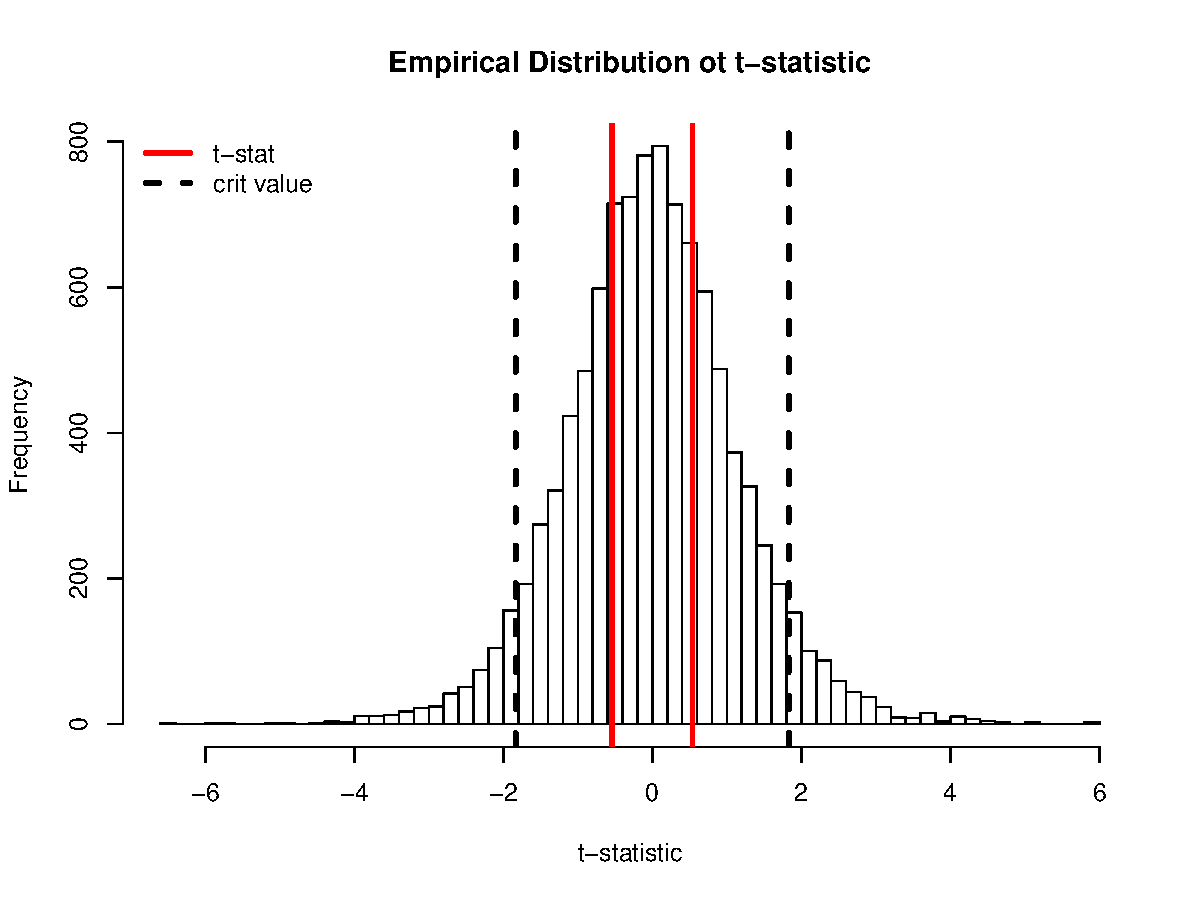
\includegraphics[trim={0cm 0cm 0cm 1.5cm}, clip, scale=0.6]{../figs/ttest_dist.pdf}
\end{minipage}
\end{figure}

\subsection{Difference in proportions (e.g. A/B testing)}

\section{Evaluating the importance of regression parameters}

\section{Conclusion}

\pagebreak
\section{References}

\end{document}
